\documentclass[11pt,compress,t,notes=noshow, aspectratio=169, xcolor=table]{beamer}

\usepackage{../../style/lmu-lecture}
% Defines macros and environments
% This file is included in slides and exercises

% Rarely used fontstyle for R packages, used only in 
% - forests/slides-forests-benchmark.tex
% - exercises/single-exercises/methods_l_1.Rnw
% - slides/cart/attic/slides_extra_trees.Rnw
\newcommand{\pkg}[1]{{\fontseries{b}\selectfont #1}}

% Spacing helpers, used often (mostly in exercises for \dlz)
\newcommand{\lz}{\vspace{0.5cm}} % vertical space (used often in slides)
\newcommand{\dlz}{\vspace{1cm}}  % double vertical space (used often in exercises, never in slides)
\newcommand{\oneliner}[1] % Oneliner for important statements, used e.g. in iml, algods
{\begin{block}{}\begin{center}\begin{Large}#1\end{Large}\end{center}\end{block}}

% Don't know if this is used or needed, remove?
% textcolor that works in mathmode
% https://tex.stackexchange.com/a/261480
% Used e.g. in forests/slides-forests-bagging.tex
% [...] \textcolor{blue}{\tfrac{1}{M}\sum^M_{m} [...]
% \makeatletter
% \renewcommand*{\@textcolor}[3]{%
%   \protect\leavevmode
%   \begingroup
%     \color#1{#2}#3%
%   \endgroup
% }
% \makeatother


%\title{iML: Post-hoc Methods for Neural Networks}
%\subtitle{Visualizing Neural Networks}

\title{Interpretable Machine Learning}
\date{}
\begin{document}
%	\maketitle
	\graphicspath{ {./figure/} }

 
\newcommand{\titlefigure}{figure/iml-grad-nn.pdf}
\newcommand{\learninggoals}{
\item Visualizing architectural units
\item Visualizing filters in CNNs
\item Visualizing attention maps}

\lecturechapter{Visualizing Neural Networks}
\lecture{Interpretable Machine Learning}

	
\begin{frame}[c]{Inspecting the Model units}
    \begin{itemize}
        \item Neural Networks architectural units can be inspected to provide insights
        \item What happens to the input signal as it travels through the network ?
        \begin{itemize}
            \item Activations: Activation in neural networks are sparse
            \item Attention units: Encode the importance of input representation units
        \end{itemize}
    \end{itemize}
    
    \centering
    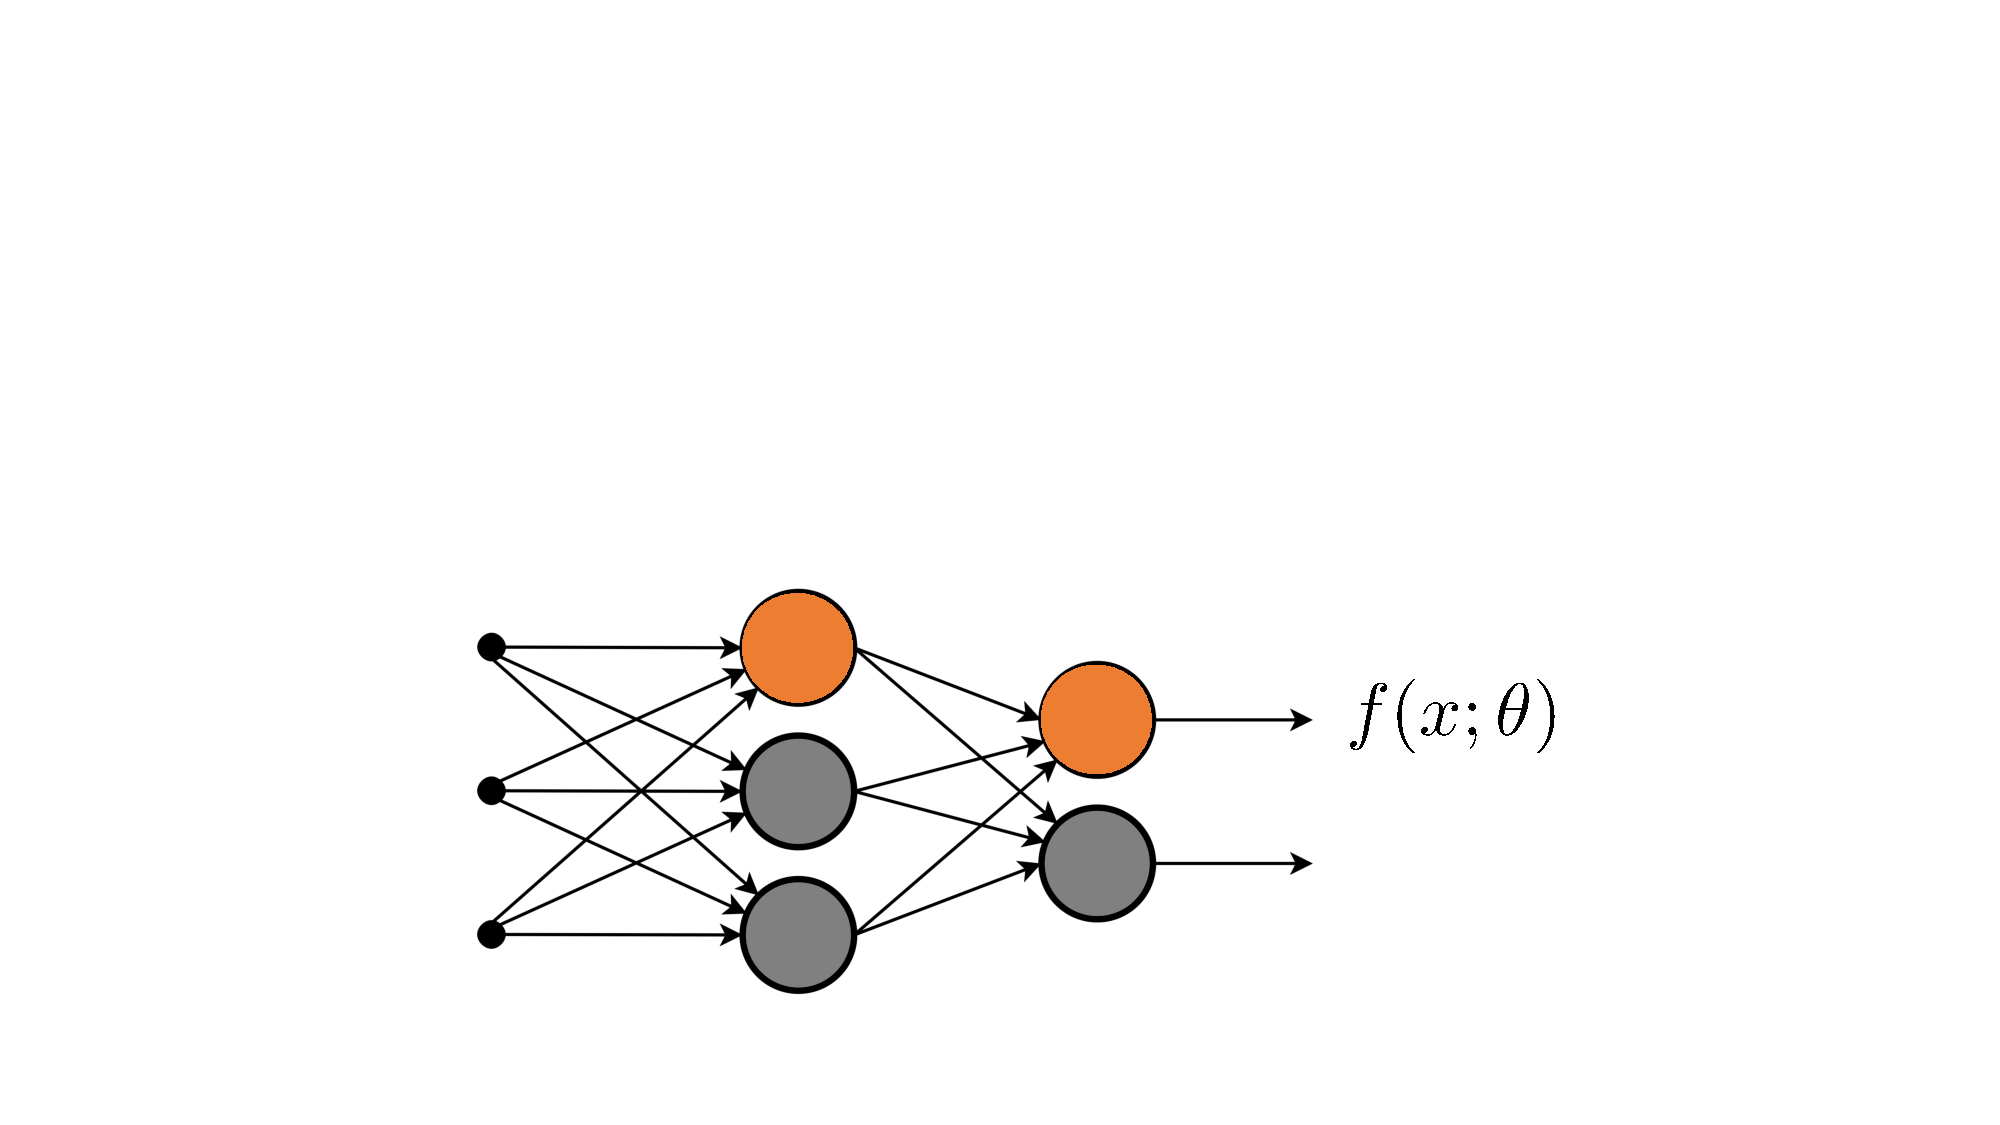
\includegraphics[scale=1]{figure/iml-grad-nn.pdf}
\end{frame}

\begin{frame}{Visualizing Neural Network Architectural Units}
    \begin{itemize}
        \item Search for examples where individual features have high values —
        \begin{itemize}
            \item Either for a neuron at an individual position, or for an entire channel
        \end{itemize}
    \end{itemize}
    
    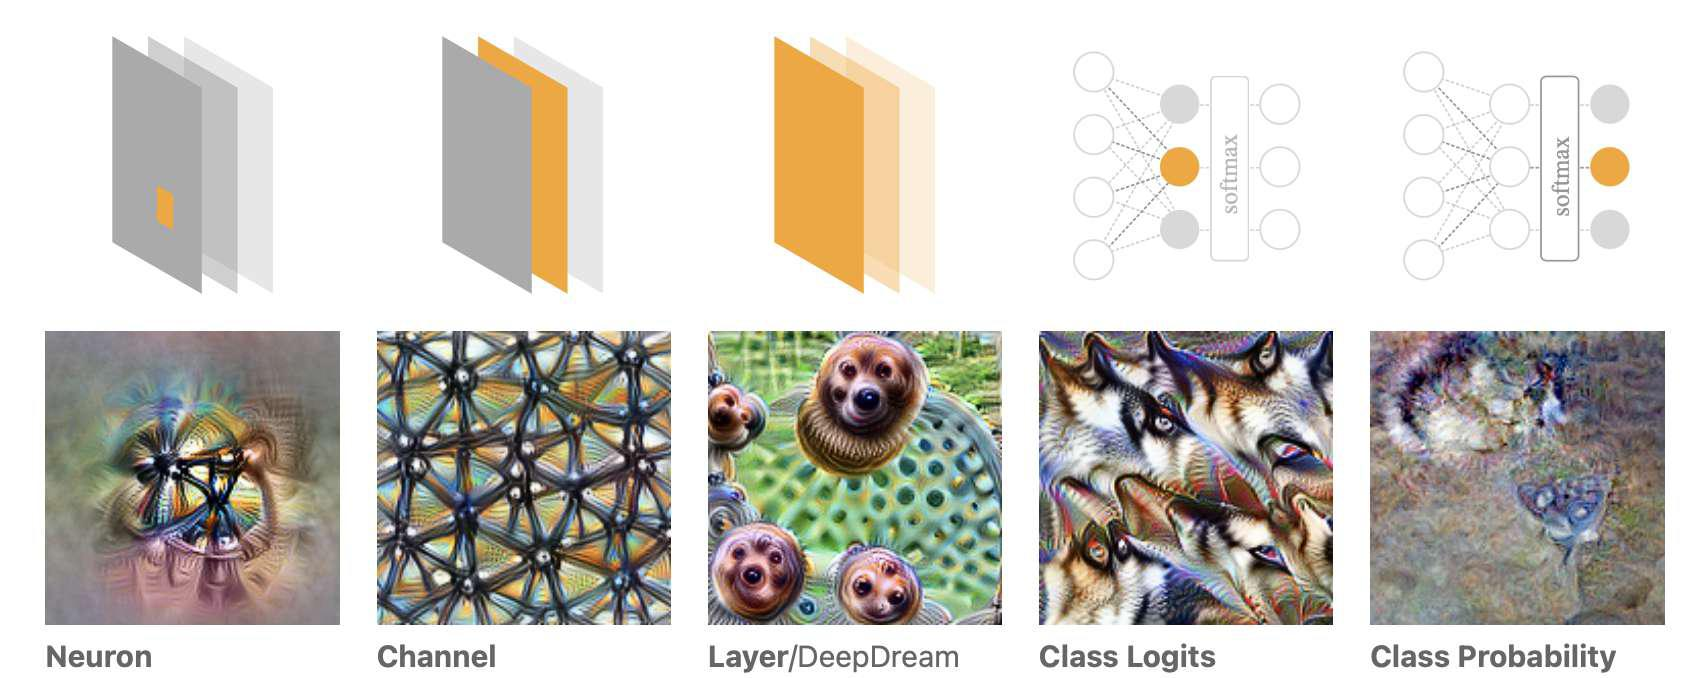
\includegraphics[scale=.47]{img180}
\end{frame}
    
\begin{frame}{Visualizing Filters in a CNN}
    \begin{itemize}
        \item Most of the aggregated values at neurons do not result in activations
        \item Find image patches in dataset that maximally activate/excite a unit
    \end{itemize}
    \begin{figure}
        \centering
        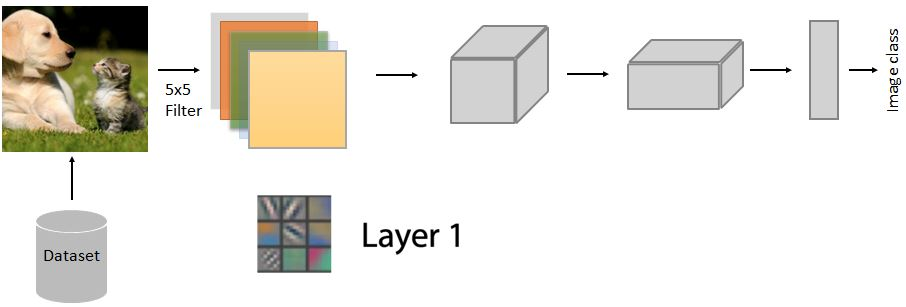
\includegraphics[scale=.6]{Bild6}
    \end{figure}
\end{frame}

	
\begin{frame}{Feature extraction evolution}
    \begin{itemize}
        \item Lower layers extract lower-level features
        \item Higher layers compose extracted features to compose high-level features
    \end{itemize}
    \begin{figure}[h]
         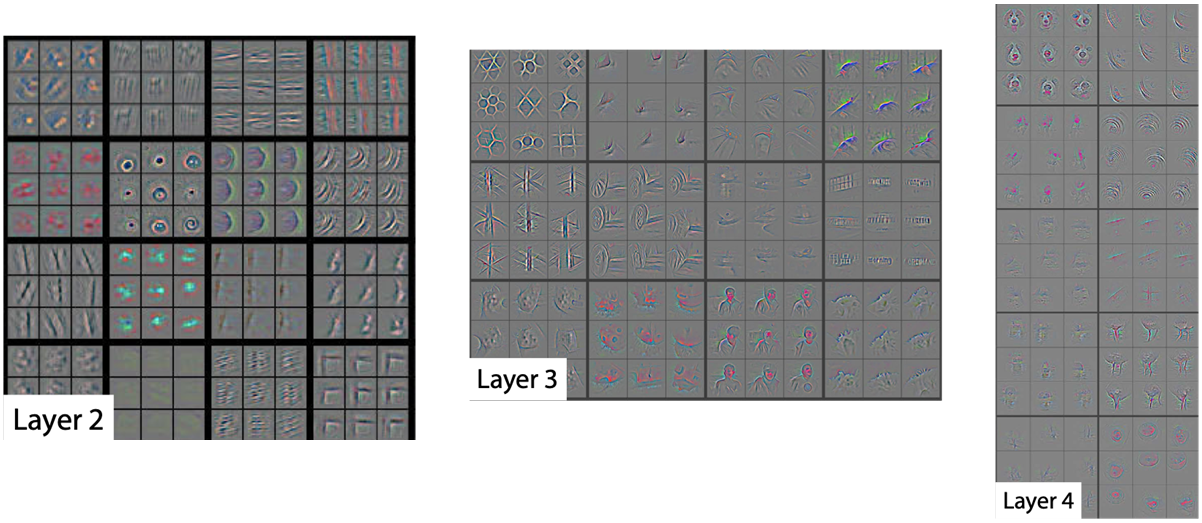
\includegraphics[scale=.4]{bild7}
    \end{figure}
\end{frame}
	
	
\begin{frame}{Layerwise Visualisation of CNNs}
    \begin{figure}
        \centering
        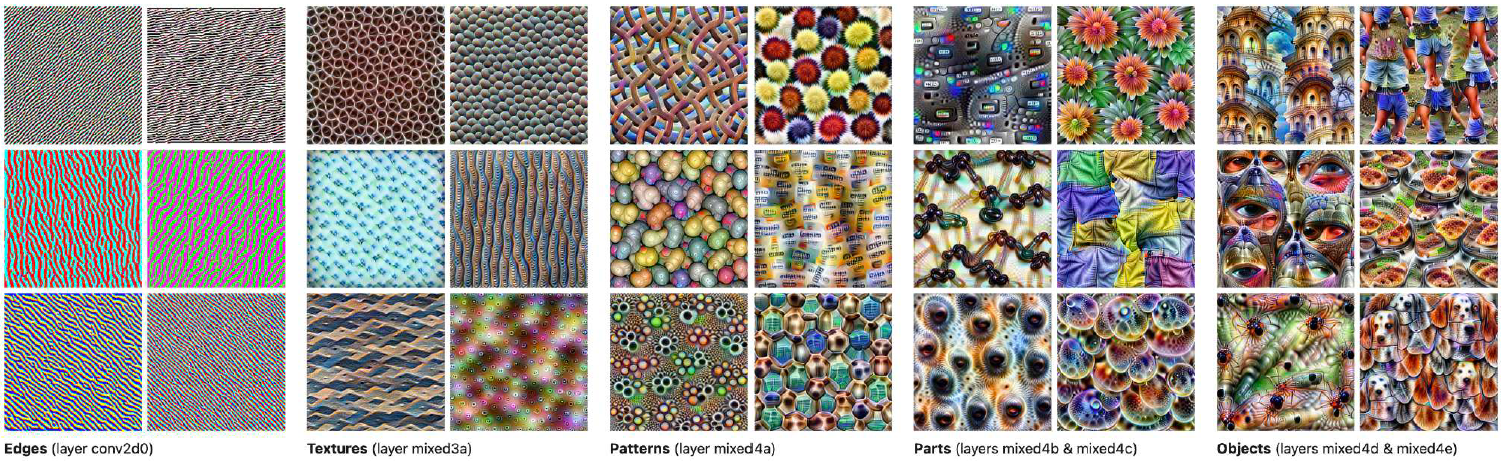
\includegraphics[scale=.38]{bild8}
    \end{figure}
\end{frame}
	
\begin{frame}{Class Activation Maps} % add the top right text
    \begin{itemize}
        \item CAMs are specific to CNNs
        \item Class activation map or CAM highlights class-specific discriminative regions
        \begin{itemize}
            \item Different classes induce different activations
        \end{itemize}
    \end{itemize}
    \begin{figure}
        \centering
        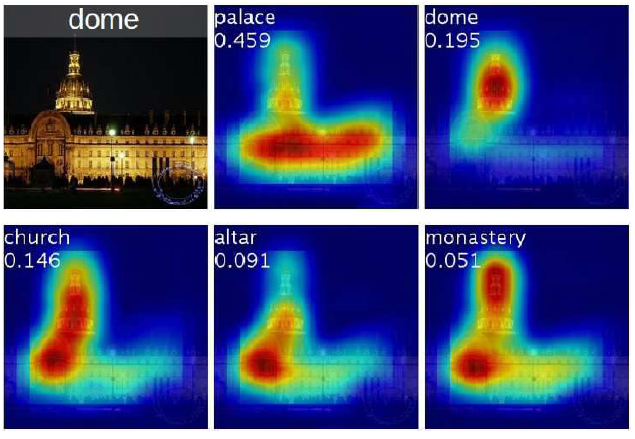
\includegraphics[width=0.5\linewidth]{bild9}
    \end{figure}
\end{frame}
	
\begin{frame}{Class Activation Maps}
    \begin{itemize}
        \item Let the activation at unit \textit{k}, at the location \textit{(x,y)} in the last layer -\textit{$f_k(x,y)$}
        \item Global avg. pooling at unit \textit{k} - $F_k$ = $\sum\limits_{x,y}f_k(x,y)$
        \item For a given class
                \begin{equation*}
                    P_c = \frac{exp(S_c)}{\sum_c exp(S_c)},\quad S_c = \sum\limits_k w_k^c F_k
                \end{equation*}
    \end{itemize}
    \begin{figure}
        \centering
        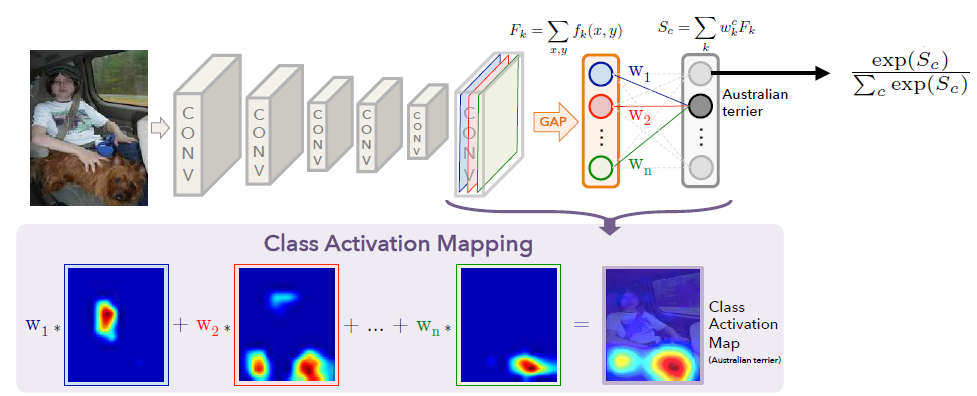
\includegraphics[width=0.6\linewidth]{bild10}
    \end{figure}
\end{frame}	
	
\begin{frame}{Class Activation Maps}
    \begin{itemize}
        \item Input: Take a pre-trained CNN model
        \item Output: weight vectors for each classes
        \item How do we learn the weights?
        \begin{itemize}
            \item Average pooling of the feature maps in the last layer
            \begin{equation*}
                S_c = \sum\limits_k w_k^c F_k
            \end{equation*}
            \item Weights learned using simple logistic regression
        \end{itemize}
    \end{itemize}
    \begin{figure}
        \centering
        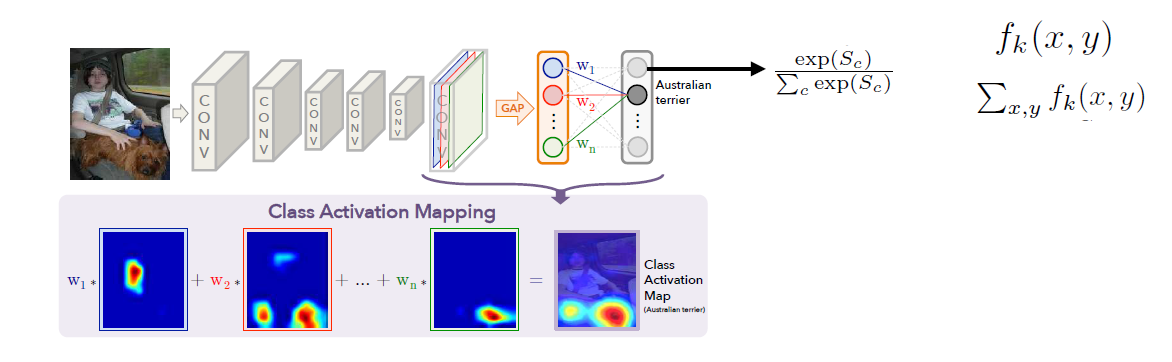
\includegraphics[scale=.35]{bild11}
    \end{figure}
\end{frame}

\begin{frame}{Attention in Language}
    \begin{itemize}
        \item Attention mechanism in neural language models is crucial for extracting latent features
        \item Self-attention in language is aimed at re-representing the initial representation based on
the context
\item Neural models consume non-contextual token-level representations and output
contextual token-level representation
    \end{itemize}
    \begin{figure}
        \centering
        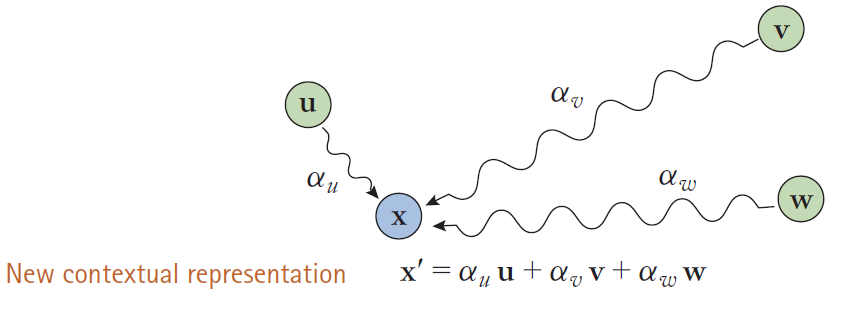
\includegraphics[width=0.4\linewidth]{bild12}
    \end{figure}
    \pause
    \begin{equation*}
        \alpha_u  = \frac{e^{sim(u,x)}}{e^{sim(u,x)} + e^{sim(v,x)} + e^{sim(w,x)}}; \quad sim(u,x) = x\cdot Wu
    \end{equation*}
\end{frame}

\begin{frame}{Attention Maps in Transformers}
\begin{figure}
    \centering
    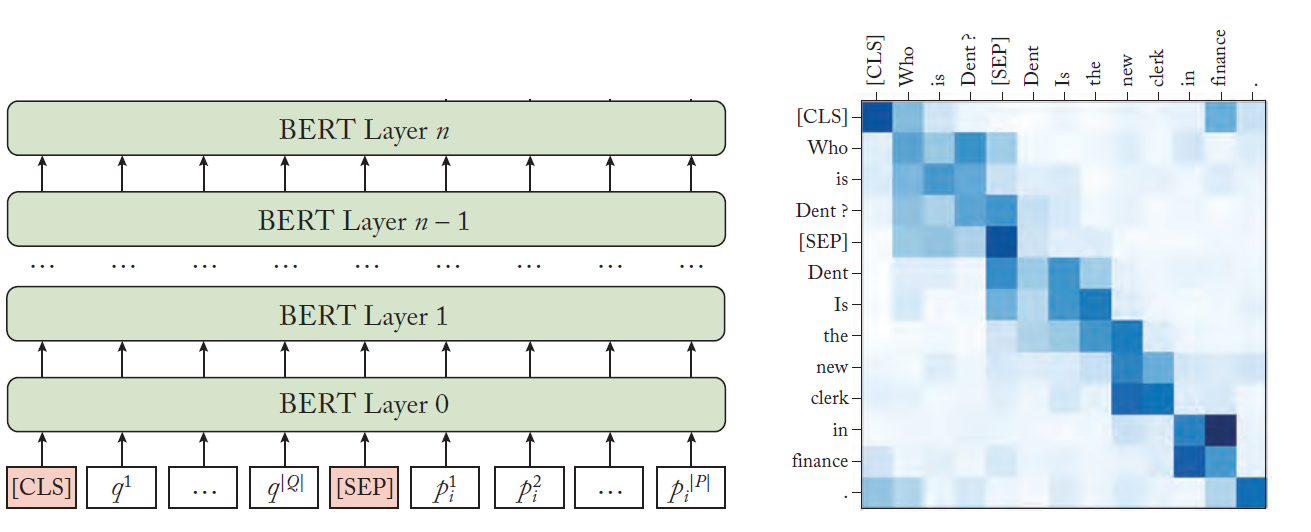
\includegraphics[scale=.4]{bild13}
\end{figure}
    
\end{frame}

\begin{frame}{Visualizing Attention Units}
    \begin{figure}
        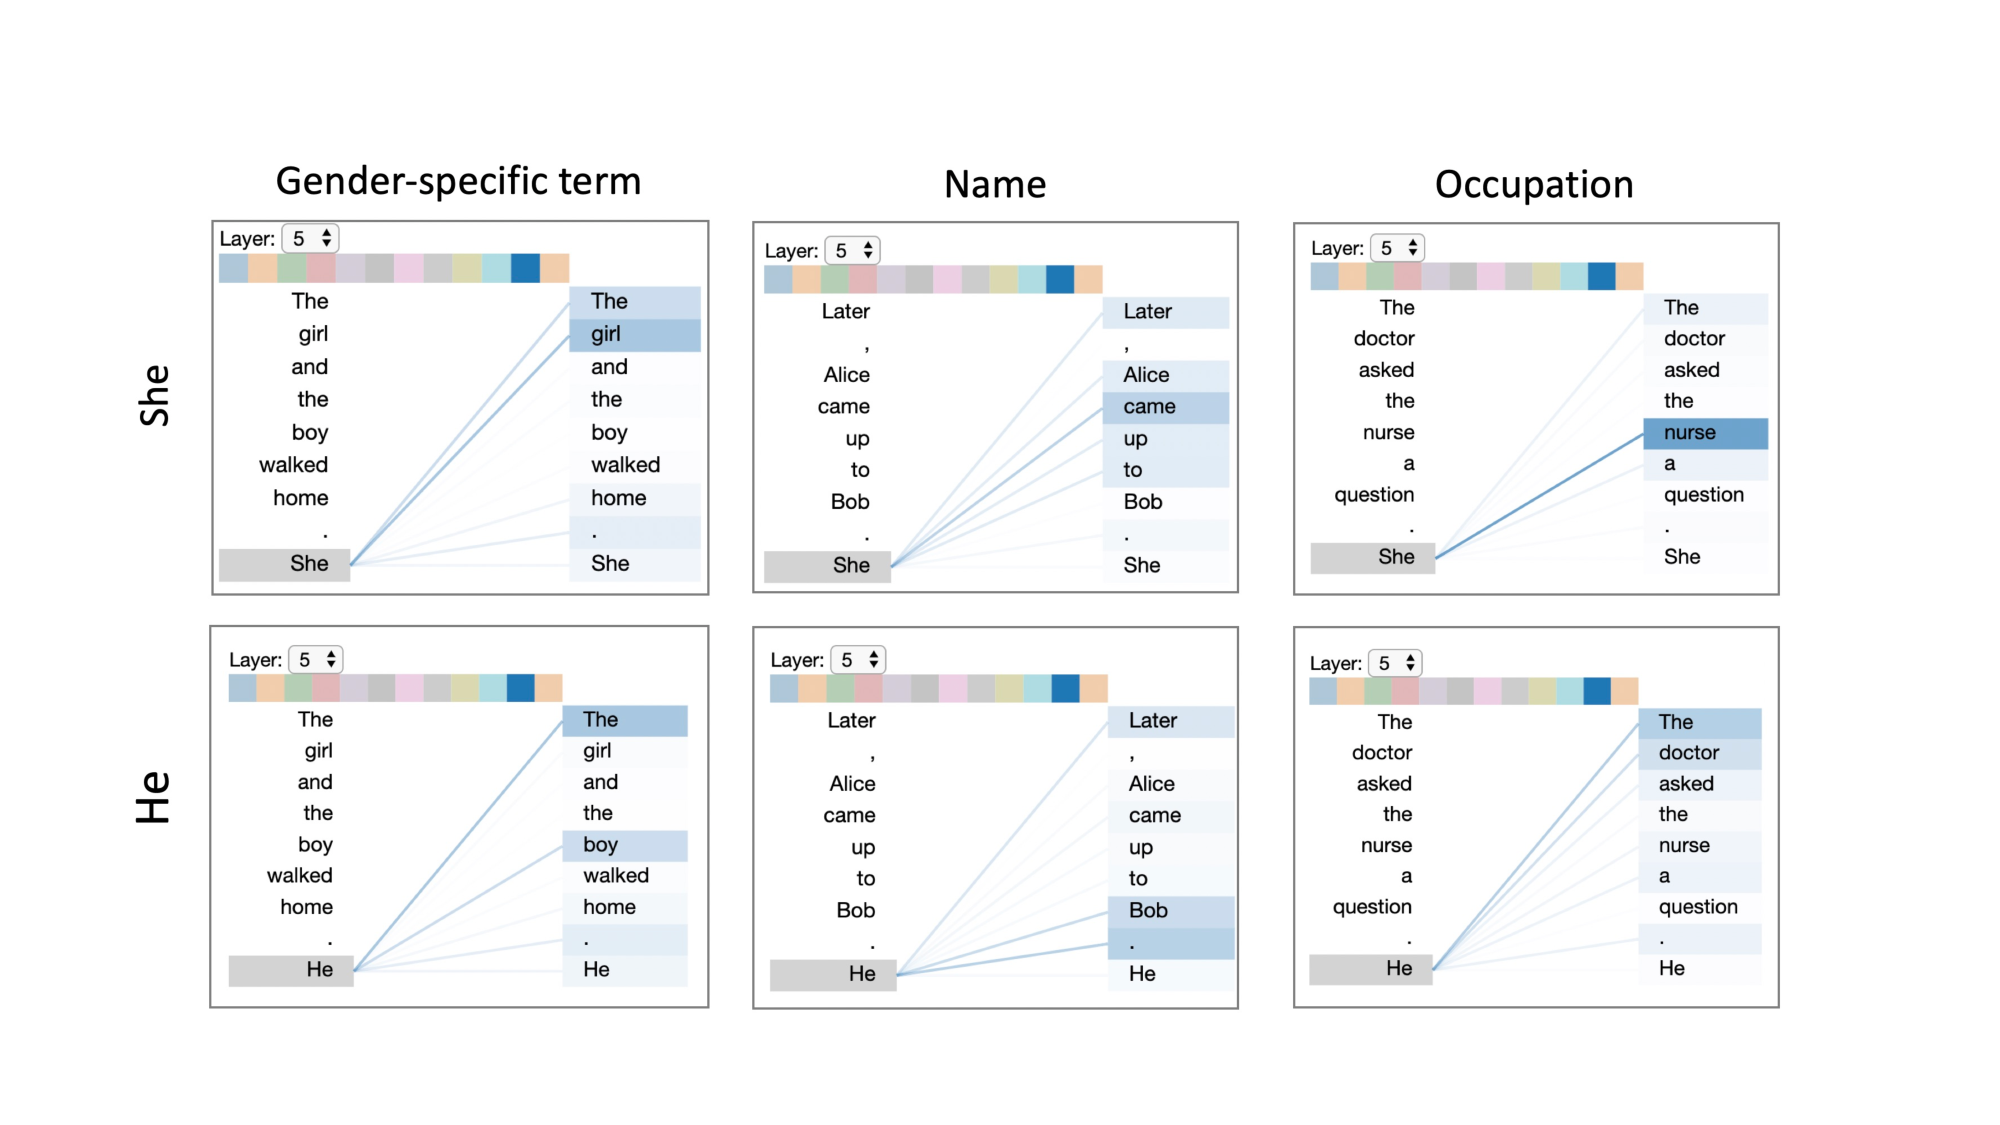
\includegraphics[scale=.45]{figure/iml-attention-vis.pdf}
    \end{figure}
\end{frame}

\begin{frame}{Other Interactive visualisations}
    \begin{itemize}
        \item Interactive visualization by Chris Olah: \url{https://distill.pub/2018/building-blocks/}
        \item \url{https://distill.pub/2017/feature-visualization/}
        \item Deep Dream
        \item De-Convolution
        \item Visualizations in Language: \url{https://github.com/jessevig/bertviz}
        \item \dots
    \end{itemize}
\end{frame}

\endlecture
\end{document}	